% Created 2017-10-27 Fri 17:25
% Intended LaTeX compiler: pdflatex
\documentclass[11pt]{article}
\usepackage[utf8]{inputenc}
\usepackage[T1]{fontenc}
\usepackage{graphicx}
\usepackage{grffile}
\usepackage{longtable}
\usepackage{wrapfig}
\usepackage{rotating}
\usepackage[normalem]{ulem}
\usepackage{amsmath}
\usepackage{textcomp}
\usepackage{amssymb}
\usepackage{capt-of}
\usepackage{hyperref}
\usepackage{amsmath}
\author{Jake Brawer}
\date{\today}
\title{Assignment 5}
\hypersetup{
 pdfauthor={Jake Brawer},
 pdftitle={Assignment 5},
 pdfkeywords={},
 pdfsubject={},
 pdfcreator={Emacs 25.2.1 (Org mode 9.1.2)}, 
 pdflang={English}}
\begin{document}

\maketitle


\section*{Problem 1}
\label{sec:orgc48955e}

\subsection*{a)}
\label{sec:org2f9eaa8}

To prove: \(E(W_{n}) = c_{b}E(W_{n - 1})\)
\begin{align}
  E(W_{n}) &= \sum_{W_{n - 1}}^{} E(W_{n} |W_{n - 1} = w_{n - 1})\\
  &= ((1 - b)w_{n-1} + 2bw_{n-1})(0.5)\\
  & \qquad+ ((1 - b)w_{n-1} + 1.4bw_{n-1})(0.5) \notag \\
  &= (1 + .2b)w_{n - 1}\\
  &= c_{b}w_{n -1}
\end{align}

Here \(c_{b}\) is maximized by when \(b = 1\).

\(E(W_{n})\) is recursively defined so:
\begin{align}
  E(W_n) &= c_{b}E(w_{n-1})\\
         &= c_{b}c_{b}E(w_{n-2})\\
         &= c_{b}c_{b}...c_{b}E(w_{n-n})\\
         &= c_{b}c_{b}...c_{b}(1) \tag{Given}\\\
         &= c_{b}^{n}
\end{align}

\subsection*{b)}
\label{sec:orgfe7b91c}

\begin{verbatim}

worth <- function(b ){
  w <- 1
  for(j in 2:1460)
  {
    if(sample(1:2, 1) == 1)
    {
      w = (1-b)*w + 2*b*w
    }
    else
    {
      w = (1-b)*w +.4*b*w
    }
  }
  return(w)
}

n <- 1000
ws <- rep(0, n)
for(i in 1:n){
  ws[i] <- worth(1)
}
hist(log10(ws))

\end{verbatim}

\begin{center}
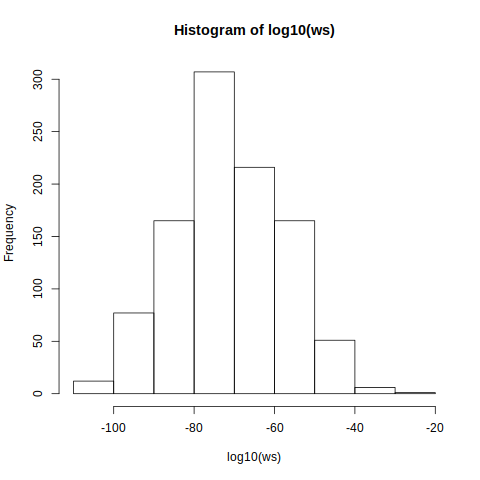
\includegraphics[width=.9\linewidth]{worth.png}
\end{center}

\subsection*{c)}
\label{sec:org105e7e1}

M_{i} =
\begin{cases}
  2 & \text{prob: } .5\\ 
  .4 & \text{prob: } .5\\ 
\end{cases}

So:\\
$\log M_{i} =$
  \begin{cases}
    .30 & \text{$M_{i}$ } $= 2$\\ 
   -.39 & \text{$M_{i}$ } $= .4$\\
  \end{cases}
\\

\text{The LLN says as} n \rightarrow \infty, \overline{L_{n}} \rightarrow E(L_{n})\\
\text{We are given: } L_{n} = X_{1} + ... + X_{n} \text{ so: }\\
\overline{L_{n}} = E(X_{1}) + ... + E(X_{n})\\
\begin{aligned}
\text{Where: } E(X_{n}) &= (.30)(.5) + (-.39)(.5)\\
&= -0.04846\\
\end{aligned}

Thus:\\
\begin{aligned}
  $\overline{L_{n}} &= n * -0.0486$ \\
  &= $ -\infty$ \text{ as n $\rightarrow \infty$}\\
\end{aligned}


\subsection*{d)}
\label{sec:org78a68cc}

\begin{align}
E(X_{n}) &= E(\log M_{i}) \notag \\
         &=  (0.5)(\log(1-.6b )\log(1 + b) ) \notag
\end{align}

Now we take the derivative of this, set to zero, and solve for b which gives us: $$b = \frac{1}{3}$$


\begin{verbatim}
ws <- rep(0, n)
for(i in 1:n){
  ws[i] <- worth(1/3)
}
hist(log10(ws))
\end{verbatim}

\begin{center}
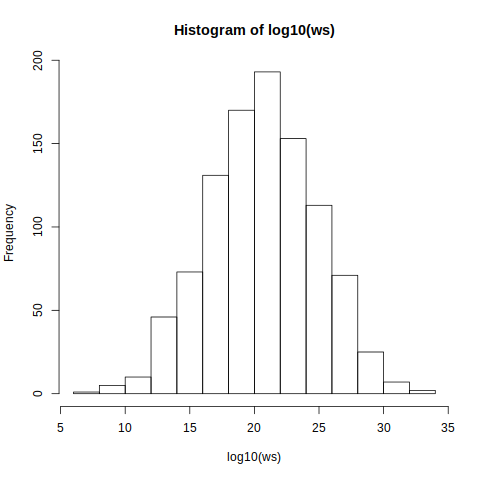
\includegraphics[width=.9\linewidth]{hist_2.png}
\end{center}

\section*{2}
\label{sec:org7a0f081}

\subsection*{a)}
\label{sec:orgad2e7a2}

By the linearity of expectation we know that: 
\begin{align}
  E(Z) &= a E(X) + b E(Y) \notag\\
       &= a \mu + b \mu \tag{Given}\\
       &= (a + b) \mu \notag
\end{align}

So in order for Z to be unbiased estimator of \(\mu\) $$ a + b = 1$$


\subsection*{b)}
\label{sec:orgc220911}

\begin{align}
  var(Z) &= a^{2}var(X) + b^{2}var(Y) \notag \\
         &= a^{2} + 4b^{2} \tag{Given.} \\
\end{align}



\section*{3}
\label{sec:org3b334c7}
\subsection*{a)}
\label{sec:org1250f07}
\begin{align}
  P\{\vline Y - \mu \vline \geq c\sigma\} &= P\{( Y - \mu )^{2} \geq c^{2}\sigma^{2}\} \notag\\
  &\leq \cfrac{E((Y - \mu)^{2})}{c^{2}\sigma^{2}} \tag{By Markov's}\\
  &= \cfrac{Var(Y)}{c^{2}\sigma^{2}} \notag\\
  &= \cfrac{1}{c^{2}n^{2}} \notag\\
  &\leq \cfrac{1}{c^{2}} \notag\\
\end{align}

\subsection*{b)}
\label{sec:org72c6e77}

$E(X)  = np = \frac{1}{6}6000 = 1000$ \\
$var(X) = np(1-p) = 6000(\frac{1}{6})(\frac{5}{6}) = 833.33$\\

$c\sigma = 100 \text{ so:}$\\
  \begin{aligned}
    c &= \frac{100}{\sigma} \notag \\
    &=\frac{100}{\sqrt[]{833.3}} \notag \\
    &= 3.464 \notag \\
    \text{Thus: } P\{| X - E(X) | \geq 100\} \leq \cfrac{1}{3.454^{2}}
  \end{aligned}

\subsection*{c)}
\label{sec:org3fdefd3}

\begin{align}
  P\{|X - E(X)| \geq 100\} &= P\{|\cfrac{X - E(X)}{\sigma}| \geq \frac{100}{\sigma}\}\\
                          &= P\{|\cfrac{X - E(X)}{\sigma}| \geq c\}\\
  \vspace{.2in}
                          &= P\{-c \leq Z \geq c\}
\end{align}

$$ P\{-c \leq Z \geq c\} = 0.00053$$

\subsection*{d)}
\label{sec:org211ecb5}

\begin{verbatim}
pbinom(900, size = 6000, prob = 1/6) +
(1 -pbinom(1100, size = 6000, prob = 1/6))
\end{verbatim}


\section*{4)}
\label{sec:org12e24e0}
\subsection*{a)}
\label{sec:org4edd87e}

X =
\begin{cases}
  0 & \text{prob: } .1\\ 
  1 & \text{prob: } .4\\ 
  2 & \text{prob: } .5\\
\end{cases}

Let Y be an r.v. representing senior parents. Y can take on a value between 0 and 6 with pmf:\\

f_{y} =
\begin{cases}
  0 & \text{prob: } .001\\ 
  1 & \text{prob: } .012\\ 
  2 & \text{prob: } .072\\
  3 & \text{prob: } .184\\ 
  4 & \text{prob: } .315\\ 
  5 & \text{prob: } .3\\
  6 & \text{prob: } .125\\
\end{cases}

\subsection*{b)}
\label{sec:org1113bad}

Let the r.v Z = X\(_{\text{1}}\) +\ldots{} +  X\(_{\text{1400}}\) where X\(_{\text{i}}\) represents how many parents student is bringing,\\
E(X) = .4 + .5(2) = 1.4\\
\begin{aligned}
  E(Z) &= E(X_{i}) + ... + E(X_{1400})\\
  &= 1.4 * 1400\\
  &= 1960
\end{aligned}

Similarly:
\begin{aligned}
  var(Z) &= var(X) * 1400\\
  &= 616 * 1400\\
  &= 8624000\\
  \text{So: } SD_{Z} = $\sqrt[]8624000{} = 24.8$
\end{aligned}


\text{Now we can find } $P\{Z \leq N\} \leq .95$ $\text{where  N is the number
  of seats we have at our disposal.}$\\

Can now plug this into R to get the answer:\\
\begin{verbatim}
# qnorm returns the number whose cumulative distribution matches the probability
# given so all we do is plug in the appropriate vals and we have our answer!
  qnorm(p=.95, mean=1960, sd=24.8)
\end{verbatim}

\begin{verbatim}
2000.7923699484
\end{verbatim}
\end{document}